\section{Theoretical Background} \label{theory}

This chapter deals with the past and present research in the relevant area which include literature review. This includes 
the significance of precise modelling of the ship's speed and its subsequent use in forecasting the ship's operation.
The theoretical background of Random Forest Regression will be discussed in this chapter 

\subsection{Literature Review}\label{litreview}

The research to estimate ship fuel consumption is an active field of research. The summary of previous research compiled by Kim et al. \cite{Kim.2021} gives a good overview of the methodology used to estimate Fuel Oil Consumption (FOC). For example, {Be{\c{s}}ik{\c{c}}i} et al. \cite{BalBesikci.2016}, Jeon et al. \cite{Jeon.2018} and Kim et al. \cite{Kim.2021} utilised ANN to estimate FOC and reported good results by comparing ANN model's performance against Multiple Linear Regression model. It will be also sensible to compare the performance of ANN model against other machine learning models. \\

The research by Gkerekos et al. \cite{Gkerekos.2019} showcased the performance of different machine learning models to predict ship's (FOC) using both noon data and automated data logging and monitoring (ADLM) system. This research concludes that Decision Tree Regressor (DTR) based model, namely Random Forest Regressor, (RFR), and Extra Tree Regressor, (ETR), displayed good prediction performance. Gkerekos et al. \cite{Gkerekos.2019} also suggested that automatic sensor based data have the potential to increase the model accuracy score, $R^2$, by $5-7\%$.\\

Li et al. \cite{Li.2022} performed a more extensive research on the effects of data fusions between meteorological data, ship voyage data and AIS data on different machine learning models to predict the ship's FOC. This research highlighted the advantage of fusing meteorological data and ship voyage data. The evaluation on different model performance indicated that RFR are among preferable model candidate to be used in commercial scale due to its good prediction capability and robustness against different datasets.\\

The research presented by Gkerekos et al. \cite{Gkerekos.2019} and Li et al. \cite{Li.2022} both used machine learning method to estimate the ship's FOC. Abebe et al. \cite{Abebe.2020} used different approach in their research by predicting the ship's Speed Over Ground (SOG) instead of FOC. Abebe et al. \cite{Abebe.2020} fused AIS satellite data and noon-report weather data for the SOG prediction. The evaluation from this research shows that machine learning methods can also be applied to predict SOG. Findings from this research also show good prediction performance of RFR.\\

This literature review indicated the capability of Random Forest Regressor to predict SOG and FOC. However, the difference of the data source as well as the data type used for modelling will result different result in model performance. From the literature review, good prediction performance from RFR can be expected. With that, this thesis will present the strength and limitations of RFR and provide general suggestions to improve the prediction performance of random forest model.\\

\subsection{Random Forest Regressor (RFR)}\label{rfrtheo}

% {Bal Be{\c{s}}ik{\c{c}}i}

\begin{figure}[h]
\centering
\begin{minipage}[b]{.5\textwidth}
    \centering
    \begin{tikzpicture}[x=0.75pt,y=0.75pt,yscale=-1,xscale=1]
    %uncomment if require: \path (0,433); %set diagram left start at 0, and has height of 433
    
    %Shape: Square [id:dp5731268858272198] 
    \draw   (180,110) -- (370,110) -- (370,300) -- (180,300) -- cycle ;
    %Straight Lines [id:da615072570759449] 
    \draw    (250,110) -- (250,300) ;
    %Straight Lines [id:da8002566967918264] 
    \draw    (300,110) -- (300,300) ;
    %Straight Lines [id:da4409034763483005] 
    \draw    (180,230) -- (250,230) ;
    %Straight Lines [id:da07514682530914596] 
    \draw    (300,170) -- (370,170) ;
    
    % Text Node
    \draw (131,192.4) node [anchor=north west][inner sep=0.75pt]    {$X_{2}$};
    % Text Node
    \draw (261,340.4) node [anchor=north west][inner sep=0.75pt]    {$X_{1}$};
    % Text Node
    \draw (157,222.4) node [anchor=north west][inner sep=0.75pt]    {$t_{2}$};
    % Text Node
    \draw (201,252.4) node [anchor=north west][inner sep=0.75pt]    {$R_{1}$};
    % Text Node
    \draw (201,162.4) node [anchor=north west][inner sep=0.75pt]    {$R_{2}$};
    % Text Node
    \draw (268,192.4) node [anchor=north west][inner sep=0.75pt]    {$R_{3}$};
    % Text Node
    \draw (321,132.4) node [anchor=north west][inner sep=0.75pt]    {$R_{4}$};
    % Text Node
    \draw (321,220.4) node [anchor=north west][inner sep=0.75pt]    {$R_{5}$};
    % Text Node
    \draw (241,310.4) node [anchor=north west][inner sep=0.75pt]    {$t_{1}$};
    % Text Node
    \draw (291,312.4) node [anchor=north west][inner sep=0.75pt]    {$t_{3}$};
    % Text Node
    \draw (381,162.4) node [anchor=north west][inner sep=0.75pt]    {$t_{4}$};
    
    \end{tikzpicture}
    
    \captionof{figure}{Example of partition space} 
    \label{fig:partitionspace}
\end{minipage}%
\begin{minipage}[b]{.5\textwidth}
    \centering
    \begin{tikzpicture}
        \tikzset{level distance=65pt,sibling distance=10pt,edge from parent/.style=
        {draw,edge from parent path={(\tikzparentnode.south)
                                -- +(0,-8pt)
                                -| (\tikzchildnode)}}}
    \Tree [.$X_1\leq t_1$ [.$X_2\leq t_2$ [.$R_1$ ] [.$R_2$ ] ]
        [.$X_1\leq t_3$ [.$R_3$ ]
        [.$X_2\leq t_4$ [.$R_4$ ] [.$R_5$ ] ] ] ]
    \end{tikzpicture}
    \captionof{figure}{Example of partition tree} 
    \label{fig:partitiontree}
\end{minipage}
\end{figure}


\begin{tikzpicture}[x=0.75pt,y=0.75pt,yscale=-1,xscale=1]
    %uncomment if require: \path (0,452); %set diagram left start at 0, and has height of 452
    
    %Shape: Axis 2D [id:dp697661158302031] 
    \draw  (220,297.8) -- (517.5,297.8)(249.75,80) -- (249.75,322) (510.5,292.8) -- (517.5,297.8) -- (510.5,302.8) (244.75,87) -- (249.75,80) -- (254.75,87)  ;
    %Image [id:dp23308396965327827] 
    \draw (245,305) node [rotate=-40.58] {
\includegraphics[width=26.87pt,height=72.39pt]{02_figures/ferry.jpg}};
    
    
    
    
\end{tikzpicture}

Suppose the following decision tree regressor


\subsection{Ship speed}


\subsection{Modelling}




